\chapter{Method}\label{ch:method}

This chapter presents a novel framework for addressing the dynamic clustering
problem. It begins with the introduction of a new class of transitions that
incorporates the recurrence of clusters over time, enabling a more realistic
modeling of evolving data streams. A new formulation of overlapping scores is
then proposed for both spherical and Gaussian clusters, allowing for an easy
thresholding for detecting overlapping between clusters. The chapter concludes
with a detailed description of the framework's architecture, outlining its
components and their interactions in supporting adaptive and interpretable
dynamic clustering.

\section{Extended Transitions}\label{sec:extended_transitions}

To more accurately capture the dynamic evolution of clusters over time, this
section introduces an extension to the traditional notion of transitions.
Instead of relying only on pairwise comparisons or aggregate statistics,
transitions are modeled using a structured and interpretable representation. As
described in MEC~\cite{mec}, one effective approach is to represent transitions
between two clustering results as a \textbf{bipartite graph}. In this graph,
each node represents a cluster at a specific time point, and edges indicate the
presence of overlap between clusters across two consecutive timestamps.

This representation enables a methodical framework for identifying and
classifying transition patterns. Each edge encodes a correspondence between
clusters, allowing the system to categorize transitions such as
\emph{survivals}, \emph{splits}, \emph{merges}, \emph{appearances}, and
\emph{disappearances}, based on the edge connectivity patterns. The resulting
graph-based model facilitates a more expressive and insightful analysis of
cluster evolution.

\begin{figure}[H]
    \centering
    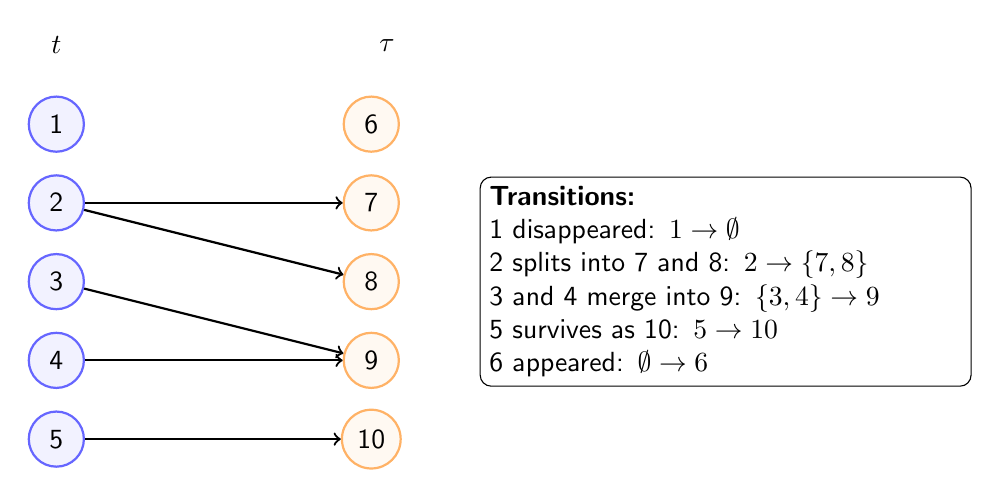
\begin{tikzpicture}[
            leftnode/.style={circle, draw=blue!60, fill=blue!5, thick, minimum size=7mm},
            rightnode/.style={circle, draw=orange!60, fill=orange!5, thick, minimum size=7mm},
            font=\sffamily,
            node distance=8mm and 30mm
        ]

        % Time labels
        \node[font=\bfseries] at (0,2) {$t$};
        \node[font=\bfseries] at (4.2,2) {$\tau$};

        % Left nodes (1 to 5)
        \node[leftnode] (n1) at (0,1) {1};
        \node[leftnode] (n2) at (0,0) {2};
        \node[leftnode] (n3) at (0,-1) {3};
        \node[leftnode] (n4) at (0,-2) {4};
        \node[leftnode] (n5) at (0,-3) {5};

        % Right nodes (6 to 10)
        \node[rightnode] (n6) at (4,1) {6};
        \node[rightnode] (n7) at (4,0) {7};
        \node[rightnode] (n8) at (4,-1) {8};
        \node[rightnode] (n9) at (4,-2) {9};
        \node[rightnode] (n10) at (4,-3) {10};

        % Edges
        \draw[->, thick] (n2) -- (n7);
        \draw[->, thick] (n2) -- (n8);
        \draw[->, thick] (n3) -- (n9);
        \draw[->, thick] (n4) -- (n9);
        \draw[->, thick] (n5) -- (n10);

        % Transitions legend centered vertically
        \node[align=left, anchor=center, text width=6cm, draw, rounded corners] (legend) at (8.5,-1) {
            \textbf{Transitions:} \\
            1 disappeared: $1 \rightarrow \emptyset$ \\
            2 splits into 7 and 8: $2 \rightarrow \{7, 8\}$ \\
            3 and 4 merge into 9: $\{3, 4\} \rightarrow 9$ \\
            5 survives as 10: $5 \rightarrow 10$ \\
            6 appeared: $\emptyset \rightarrow 6$
        };

    \end{tikzpicture}
    \caption{Example of transitions from clusters at time $t$ to clusters at time $\tau$.}
    \label{fig:cluster-transitions}
\end{figure}

To support fine-grained tracking and avoid ambiguity in complex transitions,
events such as merges and splits are decomposed into \textbf{atomic
      transitions}. Each atomic transition links a single source cluster to a
destination cluster (or vice versa), enabling a clearer interpretation of
compound transitions.

\begin{figure}[H]
    \centering
    \begin{minipage}{0.55\textwidth}
        \centering
        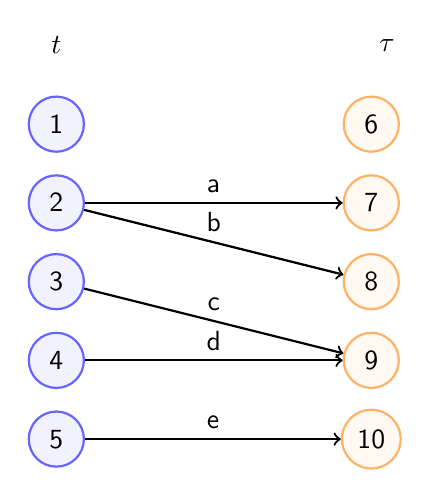
\begin{tikzpicture}[
                leftnode/.style={circle, draw=blue!60, fill=blue!5, thick, minimum size=7mm},
                rightnode/.style={circle, draw=orange!60, fill=orange!5, thick, minimum size=7mm},
                font=\sffamily,
                node distance=8mm and 30mm
            ]

            % Time labels
            \node[font=\bfseries] at (0,2) {$t$};
            \node[font=\bfseries] at (4.2,2) {$\tau$};

            % Left nodes (1 to 5)
            \node[leftnode] (n1) at (0,1) {1};
            \node[leftnode] (n2) at (0,0) {2};
            \node[leftnode] (n3) at (0,-1) {3};
            \node[leftnode] (n4) at (0,-2) {4};
            \node[leftnode] (n5) at (0,-3) {5};

            % Right nodes (6 to 10)
            \node[rightnode] (n6) at (4,1) {6};
            \node[rightnode] (n7) at (4,0) {7};
            \node[rightnode] (n8) at (4,-1) {8};
            \node[rightnode] (n9) at (4,-2) {9};
            \node[rightnode] (n10) at (4,-3) {10};

            % Edges
            \draw[->, thick] (n2) -- (n7) node[midway, above] {a};
            \draw[->, thick] (n2) -- (n8) node[midway, above] {b};
            \draw[->, thick] (n3) -- (n9) node[midway, above] {c};
            \draw[->, thick] (n4) -- (n9) node[midway, above] {d};
            \draw[->, thick] (n5) -- (n10) node[midway, above] {e};

        \end{tikzpicture}
    \end{minipage}
    \hfill
    \begin{minipage}{0.4\textwidth}
        \centering
        \begin{tabular}{|c|c|c|l|}
            \hline
            \textbf{Edge} & \textbf{From} & \textbf{To} & \textbf{Type} \\
            \hline
            -             & 1             & -           & Disappearance \\
            a             & 2             & 7           & Split         \\
            b             & 2             & 8           & Split         \\
            c             & 3             & 9           & Merge         \\
            d             & 4             & 9           & Merge         \\
            e             & 5             & 10          & Survival      \\
            -             & -             & 6           & Appearance    \\
            \hline
        \end{tabular}
    \end{minipage}
    \caption{Example of atomic cluster transitions between time $t$ and $\tau$.}
    \label{fig:atomic-cluster-transitions}
\end{figure}

The classification of transitions relies on analyzing the degree of
connectivity (i.e., number of incident edges) for each node in the bipartite
graph constructed between clustering results at times $t$ and $\tau$:

\begin{itemize}
      \item \textbf{At time $t$}:
            \begin{itemize}
                  \item A cluster with no outgoing edges is labeled as \emph{disappeared}.
                  \item A cluster with multiple outgoing edges is considered to have undergone a
                        \emph{split}.
            \end{itemize}

      \item \textbf{At time $\tau$}:
            \begin{itemize}
                  \item A cluster with no incoming edges is marked as \emph{newly appeared}.
                  \item A cluster with multiple incoming edges is the result of a \emph{merge}.
            \end{itemize}
\end{itemize}

When a cluster node at either time $t$ or $\tau$ has exactly one connecting
edge, the nature of the transition cannot be inferred directly from the graph
structure alone. In such cases, additional context is needed to disambiguate:

\begin{itemize}
      \item \textbf{From time $t$ to $\tau$}:
            \begin{itemize}
                  \item If the destination cluster has only one incoming edge, the transition is a
                        \emph{survival}.
                  \item If the destination cluster has multiple incoming edges, the source cluster has
                        \emph{merged} with others.
            \end{itemize}

      \item \textbf{From time $\tau$ to $t$}:
            \begin{itemize}
                  \item If the originating cluster has only one outgoing edge, the transition is a
                        \emph{survival}.
                  \item If the originating cluster has multiple outgoing edges, it has \emph{split}.
            \end{itemize}
\end{itemize}

When both nodes involved in a transition have exactly one edge but are each
involved in other connections, the transition is labeled as a
\textbf{mergesplit}, representing a complex reconfiguration that combines
merging and splitting behaviors.

\begin{figure}[H]
    \centering
    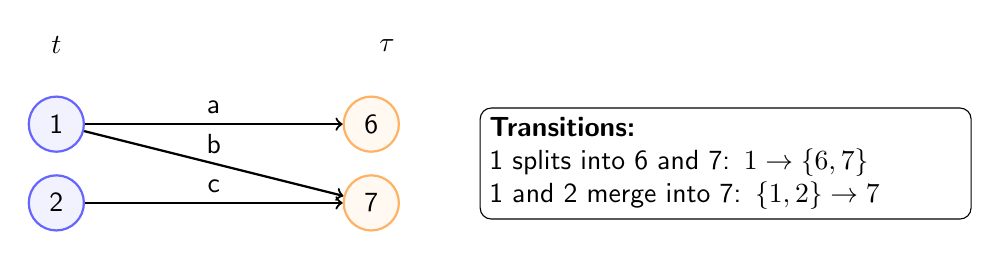
\begin{tikzpicture}[
            leftnode/.style={circle, draw=blue!60, fill=blue!5, thick, minimum size=7mm},
            rightnode/.style={circle, draw=orange!60, fill=orange!5, thick, minimum size=7mm},
            font=\sffamily,
            node distance=8mm and 30mm
        ]

        % Time labels
        \node[font=\bfseries] at (0,2) {$t$};
        \node[font=\bfseries] at (4.2,2) {$\tau$};

        % Left nodes
        \node[leftnode] (n1) at (0,1) {1};
        \node[leftnode] (n2) at (0,0) {2};

        % Right nodes
        \node[rightnode] (n6) at (4,1) {6};
        \node[rightnode] (n7) at (4,0) {7};

        % Edges
        \draw[->, thick] (n1) -- (n6) node[midway, above] {a};
        \draw[->, thick] (n1) -- (n7) node[midway, above] {b};
        \draw[->, thick] (n2) -- (n7) node[midway, above] {c};

        % Legend (left)
        \node[align=left, anchor=center, text width=6cm, draw, rounded corners] (legend) at (8.5,0.5) {
            \textbf{Transitions:} \\
            1 splits into 6 and 7: $1 \rightarrow \{6, 7\}$ \\
            1 and 2 merge into 7: $\{1, 2\} \rightarrow 7$
        };

    \end{tikzpicture}

    \vspace{1em}

    % Table below the diagram
    \begin{minipage}{0.8\textwidth}
        \centering
        \begin{tabular}{|c|c|c|l|}
            \hline
            \textbf{Edge} & \textbf{From} & \textbf{To} & \textbf{Transition Type} \\
            \hline
            a             & 1             & 6           & Split                    \\
            b             & 1             & 7           & Mergesplit               \\
            c             & 2             & 7           & Merge                    \\
            \hline
        \end{tabular}
    \end{minipage}
    \caption{Example of a mergesplit transition.}
    \label{fig:cluster-mergesplit}
\end{figure}

While the transitions discussed so far describe short-term structural changes
between consecutive timestamps, long-term dynamics often involve recurring
patterns. To support extended temporal analysis, three additional transition
types are introduced: \textbf{reappearance}, \textbf{remerge}, and
\textbf{resplit}.

\begin{itemize}
      \item \textbf{Reappearance}: A cluster that previously disappeared
            re-emerges after some delay. Formally, let $C_i^t$ be a cluster
            such that $C_i^t \rightarrow \emptyset$. Then $C_j^\tau$ with $\tau > t$
            is said to be a reappearance of $C_i^t$ if:
            \[
                  C_i^t \circledast C_j^\tau.
            \]
            This condition distinguishes reappearance from pure appearance by matching the
            new cluster to a previously disappeared one.

      \item \textbf{Remerge}: This describes the case in which a previously
            split cluster reassembles after some time. Let $C_i^t$ be a cluster
            that undergoes a split:
            \[
                  C_i^t \rightarrow \{C_1^{t+1}, \dots, C_v^{t+1}\}.
            \]
            Suppose that these clusters $\{C_1^{t+1}, \dots, C_v^{t+1}\}$ persist over time
            up to the time $\tau - 1$, retaining their identity, and eventually undergo a
            merge at time $\tau > t + 1$:
            \[
                  \{C_1^{\tau - 1}, \dots, C_v^{\tau - 1}\} \rightarrow C_j^{\tau}.
            \]
            Then $C_j^{\tau}$ is said to be a \emph{remerge} of $C_i^t$ if:
            \[
                  C_i^t \circledast C_j^{\tau}.
            \]

      \item \textbf{Resplit}: This is the converse of remerge. Let $\{C_1^t, \dots, C_u^t\}$ be clusters that were previously merged:
            \[
                  \{C_1^t, \dots, C_u^t\} \rightarrow C_i^{t+1},
            \]
            and suppose that $C_i^{t+1}$ survives up to time $ \tau - 1 $ and is later
            split at time $\tau > t+1$ into:
            \[
                  C_i^{\tau - 1} \rightarrow \{C_1^{\tau}, \dots, C_u^{\tau}\}.
            \]
            The event is identified as a \emph{resplit} if:
            \[
                  \forall j \in \{1, \dots, u\}, \quad C_j^t \circledast C_j^{\tau}.
            \]
\end{itemize}

By incorporating these extended transition types, the framework enables not
only the detection of immediate structural changes but also the identification
of long-term recurrences. This allows for a more nuanced and temporally aware
analysis of cluster evolution in dynamic environments.

\section{Overlapping Scores Definition}\label{sec:overlapping_scores}
Overlapping scores are used to quantify the degree of similarity or interaction
between two clusters. In dynamic clustering, such scores play a crucial role in
understanding cluster evolution. This section introduces two novel
formulations: one tailored for spherical clusters, and one for Gaussian
clusters with arbitrary covariance structures.

\subsubsection*{Spherical Overlapping Score}

For clusters $ C_i $ and $ C_j $ exhibiting approximately spherical geometry,
the \textbf{Spherical Overlapping Score (SOS)} is introduced to quantitatively
assess their spatial proximity:

\begin{equation}\label{eq:sos}
      \text{SOS}(C_i, C_j) = 2^{- \frac{||\boldsymbol{\mu}_i, \boldsymbol{\mu}_j||_2}{r_i + r_j}}
\end{equation}

where:
\begin{itemize}
      \item $||\boldsymbol{\mu}_i - \boldsymbol{\mu}_j||_2$ denotes the Euclidean distance between the centers
            (means) $\boldsymbol{\mu}_i$ and $\boldsymbol{\mu}_j$ of clusters $C_i$ and $C_j$, respectively,
      \item $r_i$ and $r_j$ are the estimated radii of clusters $C_i$ and $C_j$,
      \item The denominator $(r_i + r_j)$ serves to normalize the distance by the combined
            scale of the clusters,
      \item The exponential form ensures that SOS values lie in $(0, 1]$, decaying smoothly
            as clusters become more distant.
\end{itemize}

\textbf{Properties and Interpretation:}
\begin{itemize}
      \item The score is bounded in $ (0, 1] $, where:
            \begin{itemize}
                  \item $ \text{SOS} \to 0 $: the clusters are very distant i.e., $ ||\boldsymbol{\mu}_i, \boldsymbol{\mu}_j||_2 \rightarrow \infty $.
                  \item $ \text{SOS} = 0.5 $: the clusters are tangent, i.e., $ ||\boldsymbol{\mu}_i, \boldsymbol{\mu}_j||_2 = r_i + r_j $.
                  \item $ \text{SOS} = 1 $: the clusters are completely overlapped, i.e., $ ||\boldsymbol{\mu}_i, \boldsymbol{\mu}_j||_2 = 0 $.
            \end{itemize}

      \item The score decays exponentially with the normalized inter-cluster distance,
            providing a \emph{scale-invariant} measure of similarity.

      \item The score can be interpreted as a \textbf{probability-like value} quantifying
            the likelihood that two clusters are evolutionarily related. The most uncertain
            case is when the clusters are tangent ($ \text{SOS} = 0.5 $), where:
            \begin{itemize}
                  \item $ C_j $ could be the evolution of $ C_i $ with a large center shift,
                  \item or $ C_j $ could represent a newly formed cluster that emerged near $ C_i $.
            \end{itemize}

      \item Thanks to these properties, a natural threshold for deciding overlap is $
                  \varepsilon = 0.5 $: scores above this suggest potential continuity or evolution;
            scores below indicate separation.

      \item The score requires only the cluster centers and radii to compute, which makes
            it particularly suitable for \textbf{streaming clustering frameworks} where
            retaining all data points is infeasible. This supports lightweight and
            efficient computation.
\end{itemize}

\subsubsection*{Effective Overlapping Score for Gaussian Clusters}

Building upon the idea of the \emph{Spherical Overlapping
      Score}~(\ref{eq:sos}), which assumes spherical symmetry, the \textbf{Effective
      Overlapping Score (EffectiveOS)} generalizes the concept to clusters modeled as
multivariate Gaussian distributions. This allows for the consideration of
directional variability and correlated features by incorporating covariance
structure into the overlap estimation.

The \textbf{EffectiveOS} is defined as:

\begin{equation}
      \text{EffectiveOS} = 2^{\frac{-d_M(\boldsymbol{\mu}_i, \boldsymbol{\mu}_j)}{\text{RMSSize}_i + \text{RMSSize}_j}}
\end{equation}

where $ d_M(\boldsymbol{\mu}_i, \boldsymbol{\mu}_j) $ is the Mahalanobis distance between the cluster
means:

\begin{align}
      d_M(\boldsymbol{\mu}_i, \boldsymbol{\mu}_j) & = \sqrt{(\boldsymbol{\mu}_i - \boldsymbol{\mu}_j)^\top \Sigma_{ij}^{-1} (\boldsymbol{\mu}_i - \boldsymbol{\mu}_j)} \\
      \Sigma_{ij}       & = \frac{\Sigma_i + \Sigma_j}{2}
\end{align}

The term $ \text{RMSSize}_i $ represents the \textbf{root mean square size} of
cluster $ C_i $, capturing its generalized radius along principal directions:

\begin{align}
      \text{RMSSize}_i & = \sqrt{\frac{1}{d} \sum_{\ell=1}^d a_\ell^2} \\
      a_\ell           & = \chi^2_\alpha \sqrt{\lambda_\ell^i}
\end{align}

where:
\begin{itemize}
      \item $ \lambda_\ell^i $ are the eigenvalues of the covariance matrix $ \Sigma_i $,
            representing the variance along each principal axis of cluster $ C_i $,
      \item $ d $ is the dimensionality of the data,
      \item $ \chi^2_\alpha $ is the critical value of the chi-squared distribution at
            confidence level $ \alpha $, used to scale the eigenvalues to a desired confidence boundary.
\end{itemize}

\textbf{Properties and Intuition:}
\begin{itemize}
      \item \textbf{Generalization of Spherical Case:} When covariance matrices are multiples
            of the identity, the Mahalanobis distance reduces to the Euclidean distance, and
            RMSSize approximates the radius, thus reducing to the SOS formulation.
      \item \textbf{Covariance-aware Distance:} The Mahalanobis distance accounts for
            feature correlation and direction-dependent spread, making it suitable for ellipsoidal clusters.
      \item \textbf{Confidence-aware Scaling:} RMSSize uses the eigenvalue spectrum scaled
            by a chi-squared factor to describe the effective spatial extent of a Gaussian cluster
            with statistical rigor.
      \item \textbf{Probabilistic Interpretation:} Like SOS, the EffectiveOS is bounded
            in $ (0, 1] $ and can be interpreted as a probability-like measure of overlap or evolution
            likelihood.
      \item \textbf{Streaming-Friendly Implementation:} Although more complex than the SOS,
            the EffectiveOS still relies only on statistical summaries (means, covariances, and eigenvalues),
            making it applicable in streaming scenarios..
\end{itemize}

\section{Proposed Framework}\label{sec:proposed_framework}

The architecture of the proposed dynamic clustering framework is illustrated in
Figure~\ref{fig:architecture}. It consists of multiple interconnected modules,
each dedicated to a specific aspect of processing and tracking clusters within
a data stream.

The streaming clustering component employs the CluStream
algorithm~\cite{clustream}, which supports distinct online and offline
clustering phases and allows the offline phase to be triggered on demand. Each
submodule, namely online, offline, and triggering, is also explicitly
represented.

The original algorithm's offline phase uses K-means with a fixed number of
clusters $ k $. In contrast, the offline phase is implemented using Gaussian
Mixture Models (GMMs)~\cite{gaussian_mixtures}, where the number of components
is determined based on the Silhouette metric. This approach helps relax the
spherical cluster assumption inherent in K-means and allows the number of
clusters to adapt to the underlying data distribution without requiring prior
knowledge of $ k $.

It is noted that in the original CluStream algorithm, the offline phase is
triggered based on a fixed time interval. As previously
stated,~\cite{namitha_dynamic_clustering_2} implements a mechanism that
triggers the offline phase using the Page-Hinkley algorithm~\cite{page_hinkley}
to monitor the distance between incoming data points and their closest
microclusters.

In the present implementation, consistent with the original CluStream
algorithm, the offline phase is triggered after processing a fixed-size window
of incoming data points. This approach ensures regular macroclustering updates
while maintaining computational simplicity and avoiding the overhead associated
with more complex monitoring strategies. Thanks to the modular nature of the
proposed dynamic clustering framework, this triggering mechanism can be easily
replaced or extended to accommodate alternative strategies, such as adaptive or
data-driven methods.

Moreover, coherently with the drift detection setup, the system distinguishes
between a reference phase and a production phase. During the reference phase, a
clean, stable portion of the data is used to initialize the model. In this
stage, the deletion of microclusters is disabled to preserve the structure of
the reference distribution. Additionally, the triggering mechanism is called
only once at the end of the reference window to generate an initial
macroclustering. Once the production phase begins and new data starts streaming
in, the triggering strategy is applied at regular fixed-size intervals,
allowing the macroclustering to adapt over time.

To better understand the workflow and responsibilities within the framework,
the following paragraphs describe the core modules and their roles:

\paragraph{Online Phase (Microclustering):} The online module handles real-time summarization of the stream into
microclusters. A microcluster is a compact structure that captures summary
statistics (e.g., count, linear sum, and squared sum) of nearby data points in
the feature space. This process compresses the incoming data into a manageable
set of meaningful summaries while preserving essential distributional
characteristics. It ensures that data is processed with low latency and
prepares it for more complex downstream analysis.

\paragraph{Triggering Strategy:} Since performing macroclustering at every step would be inefficient, this
module decides when to invoke the offline phase. It monitors the evolution of
microclusters and can be based on fixed time intervals, statistical change
detection or other metric. The triggering strategy ensures a balance between
computational efficiency and responsiveness to changes in the data.

\paragraph{Offline Phase (Macroclustering):} When triggered, this module clusters the current set of microclusters to
produce macroclusters that are higher-level structures that summarize broader
data trends. Algorithms such as K-Means or Gaussian Mixture Models may be
applied to the centers of microclusters. This step extracts interpretable
patterns from the stream and forms the basis for cluster tracking.

\paragraph{History:} This module is specifically responsible for maintaining minimal yet sufficient
information about past macroclusters in order to detect complex long-term
transitions, namely \emph{reappearance}, \emph{remerge}, and \emph{resplit}.
Instead of storing the full stream or detailed cluster content, it archives
only essential descriptors (such as centroids, radii or covariance matrices,
and timestamps) of disappeared or transformed clusters. This historical memory
allows the tracking module to compare newly formed clusters with previous ones
and identify structural recurrences, enabling a deeper understanding of
temporal cluster dynamics.

\paragraph{Tracking:} The tracking module compares macroclusters across time to monitor their
evolution. It computes overlap scores using \emph{SOS} for spherical clusters
of \emph{EffectiveOS} for Gaussian-shaped clusters. Based on these scores, the
module identifies the transitions by evaluating how clusters relate to one
another temporally. This information enables the reconstruction of cluster
histories, facilitating the interpretation of dynamic patterns and structural
changes within evolving data.

\begin{figure}[H]
    \centering
    \begin{tikzpicture}[node distance=1.5cm and 2cm, every node/.style={font=\small}]
        % Nodes
        \node (stream) [diamond, draw, minimum height=0.1cm, minimum width=5cm, above, inner sep=0pt] {Streaming Data};

        \node (online) [rectangle, draw, rounded corners, text centered, minimum height=1cm, below=2cm of stream] {\shortstack{Online\\(Microclustering)}};

        \node (offline) [rectangle, draw, rounded corners, text centered, minimum height=1cm, below=of online] {\shortstack{Offline\\(Macroclustering)}};

        \node (trigger) [rectangle, draw, rounded corners, text centered, minimum height=1cm, right=of online] {Triggering Strategy};

        \node (tracking) [rectangle, draw, rounded corners, text centered, minimum height=1cm, below=of offline] {Tracking};

        \node (history) [ellipse, draw, text centered, minimum height=1cm, left=of tracking] {History};

        \node (report) [diamond, draw, text centered, minimum height=1cm, minimum width=4cm, below=2cm of tracking] {Report};

        % Arrows
        \draw[thick,->,>=stealth] (stream) -- (online);
        \draw[thick,->,>=stealth] (online) -- (offline);
        \draw[thick,->,>=stealth] (trigger) |- (offline);
        \draw[thick,->,>=stealth] (offline) -- (tracking);
        \draw[thick,->,>=stealth] (offline) -| (history);
        \draw[thick,->,>=stealth] (history) -- (tracking);
        \draw[thick,->,>=stealth] (tracking) -- (report);

        % Box
        \node[draw, dashed, inner sep=10pt, fit=(online)(offline)(trigger), label=above right:Streaming Clustering] {};
        \node[draw, dashed, inner sep=45pt, fit=(online)(offline)(trigger)(history)(tracking), label=below left:Dynamic Clustering] {};

    \end{tikzpicture}
    \caption{Proposed architecture for the dynamic clustering framework.}
    \label{fig:architecture}
\end{figure}


Together, these modules enable a flexible, efficient, and adaptive clustering
framework capable of capturing evolving patterns in streaming data while
maintaining interpretability and scalability.

The final \textbf{Report}, consolidates the output of the entire framework into
a comprehensive summary. It includes:
\begin{itemize}
      \item A graph-based visualization of transitions across all time points, extending
            the bipartite structure into a multi-step representation.
      \item A spatial visualization of the macrocluster evolution across iterations,
            showing changes in position and shape over time.
      \item A curated collection of representative data samples for each cluster at each
            timestamp.
\end{itemize}

This reporting structure not only aids in interpretation and debugging but
also enables users to analyze the evolution of data structures and validate the
clustering process both qualitatively and quantitatively.